\section{Implementation and Evaluation}
\label{Sec:Eval}


\newcommand{\golem}{\textsc{Golem}\xspace}
\newcommand{\opensmt}{\textsc{OpenSMT}\xspace}
\newcommand{\sna}{\textsc{SNA}\xspace}
\newcommand{\snaTerm}{\textsc{ItpTig}\xspace}
\newcommand{\snaOpt}{\textsc{ItpTig+}\xspace}
\newcommand{\LoAT}{\textsc{LoAT}\xspace}
\newcommand{\KoAT}{\textsc{KoAT}\xspace}
\newcommand{\Tt}{\textsc{T2}\xspace}

This section presents the implementation details and experimental 
evaluation of our approach.

\subsection{Implementation}


We implemented the prototypes of Algorithms~\ref{Alg:SNA}, \ref{Alg:SNA_Term}, and \ref{Alg:SNA_Refined} inside of \golem; 
we refer to these implementations as \sna, \snaTerm and \snaOpt.
\golem was chosen because it supports multiple different safety verification procedures,
such as Property-Directed Reachability~\cite{DBLP:journals/fac/BradleyM08} (PDR), Transition Power Abstraction~\cite{DBLP:conf/tacas/BlichaFHS22} (TPA), and Interpolation-based Model Checking~\cite{DBLP:conf/cav/McMillan03}.
Additionally, we used quantifier elimination, already implemented in \golem.
% \snaOpt with different safety verification engines was able to solve different 
% termination problems uniquely.
% Quantifier Elimination is produced by executing Model Based Projections, untill the whole formula is covere
%
For SMT queries and interpolation, our implementation uses the \opensmt  solver~\cite{DBLP:conf/sat/HyvarinenMAS16,DBLP:conf/tacas/BruttomessoPST10}.
\opensmt is integrated within \golem and provides native support for interpolation.


\subsection{Evaluation}


We compared \snaOpt against \sna and \snaTerm to evaluate the combining termination and nontermination analyses.
Additionally, we evaluated \snaOpt against several state-of-the-art tools: 
\LoAT~\cite{10.1007/978-3-031-90660-2_13} (version eacb74b), \KoAT~\cite{10.1007/978-3-031-90660-2_13} 
(version 41cb681), \Tt~\cite{DBLP:conf/tacas/BrockschmidtCIK16} (version 10f1373). 
The evaluation focused on termination analysis of Integer Transition Systems. 
Experiments were conducted on Ubuntu 20.04 machine with an AMD EPYC 7452 32-core processor and 8x32 GiB RAM. 
Our evaluation addressed the following research questions:
\begin{itemize}
\item \textbf{RQ1:} How does extending \sna with the termination procedure affect verification performance?
\item \textbf{RQ2:} How does \snaOpt perform compared to state-of-the-art tools?
\end{itemize}

The benchmark suite of Integer Transition Systems was taken from the Termination Competition~\cite{DBLP:conf/cade/GieslMRTW15}. 
Overall, there are 1222 benchmarks (538 nonterminating, 665 terminating, and 19 unknown). 
We excluded 42 trivially terminating benchmarks from the evaluation (termination of which can be detected by trivial syntactic checks), which
are solved by all tools.
The evaluation was executed with the 120 seconds timeout (the increase of the timeout does not 
significantly influence the evaluation).

\begin{table}[t!]
    \centering
    \caption{Comparison of \snaOpt with \sna and \snaTerm.}
    \label{tab:internal}
    \begin{tabular}{|c|c|c|c|c|}
        \hline
        \textbf{Algorithm} & \textbf{Total} & \textbf{Terminating} & \textbf{Nonterminating} & \textbf{Uniquely} \\
        \hline
        \sna & 343 & 0 & 343 & 7 \\
        \hline
        \snaTerm & 521 & 186 & 335 & 7 \\
        \hline
        \snaOpt & 761 & 320 & 441 & 240 \\
        \hline
    \end{tabular}
\end{table}
% \begin{figure}[t]
%     \centering
%     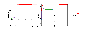
\includegraphics[width=1\linewidth]{Figures/TermCompCMP.pdf}
%     \caption{Comparison of \snaOpt with \sna and \snaTerm. The left plot is solved terminating instances, the right is nonterminating.}
%     \label{fig:golemComp}
% \end{figure}

Table~\ref{tab:internal} gives the experimental results for \snaOpt, \sna, and \snaTerm. 
It confirms that \snaOpt consistently outperforms both \sna and \snaTerm for terminating 
and nonterminating instances, solving 240 instances solved by neither \sna nor \snaTerm. 
We attribute this to the \snaOpt's generation of focused sub-problems, 
which allows the analysis to concentrate on specific reachable states.
This benefits the recurrent set detection by focusing the analysis on specific states not covered by the transition invariant.
It also benefits termination proving by extending the transition invariant with additional disjuncts 
that cover different regions of the reachable state space.
In answer to \textbf{RQ1}, the combination of termination and nontermination reasoning in 
\snaOpt significantly outperforms either individual approach in isolation.

Interestingly, \snaOpt behaves differently depending on the underlying  Safety Verification engine:
with TPA it solved 761 instances and
with PDR -- 756.
That said, it solved 22 (resp. 17) benchmarks uniquely with TPA (resp. PDR).
%

\begin{figure*}[t!]
    \centering
    \includegraphics[width=1\linewidth]{Figures/scatterSt.pdf}
    \caption{Comparison of \snaOpt with \KoAT, \LoAT and \Tt (runtime in seconds).}
    \label{fig:stateOfArtComp}
\end{figure*}

\begin{table}[t!]
    \centering
        \caption{Comparison of \snaOpt with state-of-the-art tools.}
    \label{tab:external}
    \begin{tabular}{|c|c|c|c|c|}
        \hline
        \textbf{Algorithm} & \textbf{Total} & \textbf{Terminating} & \textbf{Nonterminating} & \textbf{Uniquely} \\
        \hline
        \LoAT & 525 & 0 & 525 & 48 \\
        \hline
        \KoAT & 562 & 562 & 0 & 26 \\
        \hline
        \Tt & 1002 & 572 & 430 & 40 \\
        \hline
        \snaOpt & 761 & 320 & 441 & 8 \\
        \hline
    \end{tabular}
\end{table}

Figure~\ref{fig:stateOfArtComp} shows a scatter plot comparing \snaOpt against 
state-of-the-art termination analyzers, where each axis represents the solving time in seconds for a given tool.
Orange squares denote nonterminating instances; blue crosses denote terminating instances.
Points above the diagonal indicate instances where \snaOpt is faster than the competitor.
\snaOpt solves 761 benchmarks, with \Tt solving 1002, \KoAT 562, and \LoAT 525 instances, the full comparison can be seen in Table~\ref{tab:external}.
As shown in Figure~\ref{fig:stateOfArtComp}, \snaOpt, despite being a prototype implementation, is competitive with state-of-the-art termination analyzers.
Among all tools, \snaOpt uniquely solves eight instances (which were not solved by \sna and \snaTerm as well).
Notably, two of these — \texttt{juLinkedListCreateAddAll.jar-obl-11} and \texttt{juLinkedListCreateAddAllAt.jar-obl-17} have never been solved in the Termination Competition.
\snaOpt found recurrent sets and proved nontermination for them.
In answer to \textbf{RQ2}, \snaOpt is competitive with state-of-the-art tools and solves 
instances, not solved by any tool in the Termination Competition.
